% Generated by scripts/make_explanation_figures.py from experiment_0013 (do not edit by hand).
% Model: COVER
\documentclass[tikz,border=3pt]{standalone}
\usepackage[T1]{fontenc}
\usepackage[utf8]{inputenc}
\usepackage{newtxtext,newtxmath}
\usetikzlibrary{positioning,arrows.meta,calc}

\definecolor{neural}{HTML}{2F6DB5}
\definecolor{neuralbg}{HTML}{E8F0FA}
\definecolor{logic}{HTML}{2E8B57}
\definecolor{logicbg}{HTML}{E6F4EC}
\definecolor{relneg}{HTML}{C0392B}

\tikzset{
  tok/.style={draw=neural!80, fill=white, rounded corners=1.5pt, inner sep=1.6pt, font=\scriptsize,
              minimum height=4mm, anchor=base},
  htok/.style={tok, fill=neural!12},
  stok/.style={tok, draw=black!25, text=black!45},
  aedge/.style={line width=#1, draw=logic},
  cedge/.style={line width=#1, draw=relneg},
  ledge/.style={line width=#1, draw=neural, densely dashed},
  rlab/.style={font=\tiny, fill=white, inner sep=0.6pt},
}
\newcommand{\bars}[4]{%
  \fill[logic]  (#1-0.17,0.05) rectangle ++(0.15,{0.8*#2});
  \fill[relneg] (#1+0.02,0.05) rectangle ++(0.15,{0.8*#3});
  \node[font=\tiny, anchor=north] at (#1-0.095,0.03) {$s$};
  \node[font=\tiny, anchor=north] at (#1+0.095,0.03) {$c$};
  \node[font=\tiny, anchor=north] at (#1,-0.22) {$#2\,/\,#3$};
  \node[font=\tiny, anchor=north, text=black!60] at (#1,-0.47) {$\omega{=}#4$};
}
\newcommand{\sbar}[3]{%
  \fill[logic]  (#1-0.075,0.05) rectangle ++(0.15,{0.8*#2});
  \node[font=\tiny, anchor=north] at (#1,0.03) {$s$};
  \node[font=\tiny, anchor=north] at (#1,-0.22) {$#2$};
  \node[font=\tiny, anchor=north, text=black!60] at (#1,-0.47) {$\omega{=}#3$};
}
\providecommand{\Pcov}{P_{\mathrm{cov}}}
\providecommand{\Pnc}{P_{\neg\mathrm{conf}}}
\providecommand{\E}{\textsc{e}}
\providecommand{\N}{\textsc{n}}
\providecommand{\C}{\textsc{c}}

\begin{document}
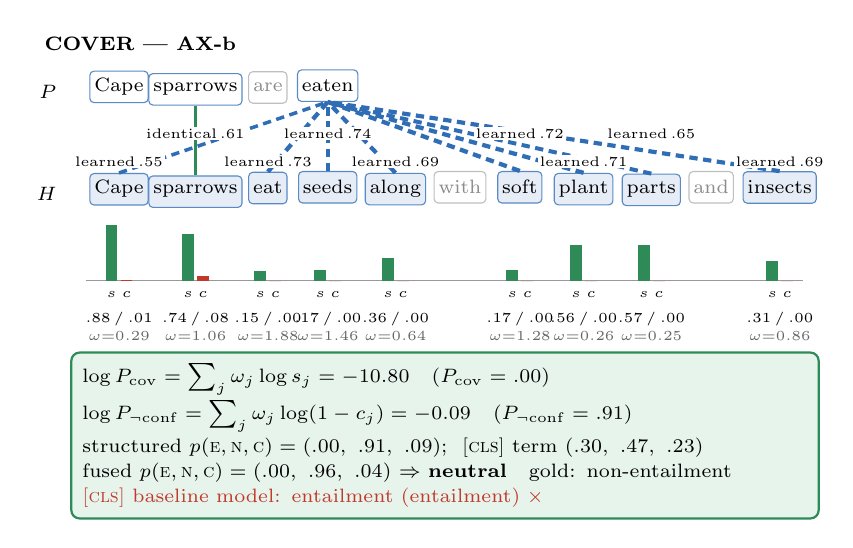
\begin{tikzpicture}
\begin{scope}[xshift=0.00cm]
\node[font=\scriptsize\itshape, anchor=east] at (-0.35,2.45) {$P$};
\node[font=\scriptsize\itshape, anchor=east] at (-0.35,1.15) {$H$};
\node[tok] (p1) at (0.32,2.45) {Cape};
\node[tok] (p3) at (1.29,2.45) {sparrows};
\node[stok] (pw2) at (2.21,2.45) {are};
\node[tok] (p7) at (2.97,2.45) {eaten};
\node[htok] (h11) at (0.32,1.15) {Cape};
\node[htok] (h13) at (1.29,1.15) {sparrows};
\node[htok] (h16) at (2.21,1.15) {eat};
\node[htok] (h17) at (2.97,1.15) {seeds};
\node[htok] (h19) at (3.83,1.15) {along};
\node[stok] (hw5) at (4.65,1.15) {with};
\node[htok] (h21) at (5.41,1.15) {soft};
\node[htok] (h22) at (6.22,1.15) {plant};
\node[htok] (h23) at (7.08,1.15) {parts};
\node[stok] (hw9) at (7.84,1.15) {and};
\node[htok] (h25) at (8.71,1.15) {insects};
\draw[ledge=1.27pt] (h11.north) -- (p7.south);
\draw[aedge=1.38pt] (h13.north) -- (p3.south);
\draw[ledge=1.56pt] (h16.north) -- (p7.south);
\draw[ledge=1.59pt] (h17.north) -- (p7.south);
\draw[ledge=1.51pt] (h19.north) -- (p7.south);
\draw[ledge=1.54pt] (h21.north) -- (p7.south);
\draw[ledge=1.53pt] (h22.north) -- (p7.south);
\draw[ledge=1.44pt] (h23.north) -- (p7.south);
\draw[ledge=1.51pt] (h25.north) -- (p7.south);
\node[rlab, anchor=south] at (0.32,1.47) {learned\,.55};
\node[rlab, anchor=south] at (1.29,1.83) {identical\,.61};
\node[rlab, anchor=south] at (2.21,1.47) {learned\,.73};
\node[rlab, anchor=south] at (2.97,1.83) {learned\,.74};
\node[rlab, anchor=south] at (3.83,1.47) {learned\,.69};
\node[rlab, anchor=south] at (5.41,1.83) {learned\,.72};
\node[rlab, anchor=south] at (6.22,1.47) {learned\,.71};
\node[rlab, anchor=south] at (7.08,1.83) {learned\,.65};
\node[rlab, anchor=south] at (8.71,1.47) {learned\,.69};
\draw[black!40] (-0.1,0.05) -- (9.01,0.05);
\bars{0.32}{.88}{.01}{0.29}
\bars{1.29}{.74}{.08}{1.06}
\bars{2.21}{.15}{.00}{1.88}
\bars{2.97}{.17}{.00}{1.46}
\bars{3.83}{.36}{.00}{0.64}
\bars{5.41}{.17}{.00}{1.28}
\bars{6.22}{.56}{.00}{0.26}
\bars{7.08}{.57}{.00}{0.25}
\bars{8.71}{.31}{.00}{0.86}
\end{scope}
\node[draw=logic, fill=logicbg, rounded corners=3pt, line width=0.8pt, font=\scriptsize, align=left, anchor=north west, text width=9.21cm, inner sep=4pt] (agg) at (-0.3,-0.85) {%
  $\log\Pcov=\sum_j\omega_j\log s_j=-10.80$\quad($\Pcov=.00$)\\[1pt]$\log\Pnc=\sum_j\omega_j\log(1-c_j)=-0.09$\quad($\Pnc=.91$)\\[1pt]structured $p(\E,\N,\C)=(.00,\ .91,\ .09)$;\ \ \textsc{[cls]} term $(.30,\ .47,\ .23)$\\[1pt]fused $p(\E,\N,\C)=(.00,\ .96,\ .04)$ $\Rightarrow$ \textbf{neutral}\quad gold: non-entailment\\[1pt]\textcolor{relneg}{\textsc{[cls]} baseline model: entailment (entailment) \texttimes}};
\node[font=\scriptsize\bfseries, anchor=south west] at (-0.75,2.85) {COVER --- AX-b};
\end{tikzpicture}
\end{document}
